\section{Datalaag}
De applicatie bevat data uit verschillende bronnen, en slaat zijn data in verschillende bronnen op. Deze data en de verbindingen met de bronnen vormen de datalaag.

\subsection{Ruwe inkomende data}

De transponderleverancier MYLAPS heeft een SDK beschikbaar gesteld aan Emando, waarmee het mogelijk is om de doorkomsten van transponders realtime binnen te krijgen. Om deze databron te benaderen bevat de datalaag een Data Collector, geïmplementeerd als Azure Cloud Worker Role, welke non-stop draait op één cloud instance. Dit proces onderhoudt de verbinding met de MYLAPS SDK.

Vanuit de MyLAPS SDK ontvangt de data laag realtime de doorkomsten van iedere transponder die langs een lus komt. Deze doorkomsten bevatten een tijdstip, een transponder nummer en een plaats op de baan. Zodra een van deze doorkomsten binnen komt, wordt deze direct opgeslagen voor toekomstig gebruik in een doorkomsten tabel in Azure Table Storage. Het kan namelijk voorkomen dat er op dit moment geen gebruiker van onze applicatie is, welke zijn transponder nummer heeft gekoppeld aan zijn account. Wanneer dit het geval is, kunnen er (nog) geen aggregaties uitgevoerd worden op deze data.

\begin{figure}[ht]
  \begin{center}
  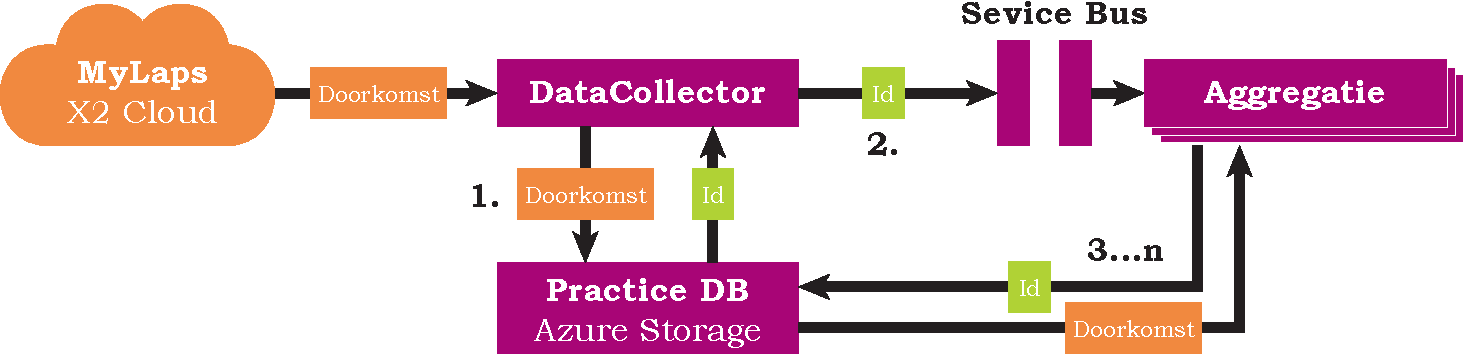
\includegraphics[width=\textwidth]{style/images/datacollector-flow}    
  \end{center}
  \caption{De werking van de Data Collector en de Service Bus}
  \label{fig:datacollector}
\end{figure}

Door deze data op te slaan, is het mogelijk om later functionaliteit in te bouwen om alsnog over deze data te kunnen aggregeren.

Nadat de data opgeslagen is, wordt via een Azure Service Bus het Id van de doorkomst doorgestuurt naar het aggregatie process in de businesslaag. Het aggregatie process raadpleegt bij het binnenkrijgen van dit Id opnieuw de doorkomst, om zo minder data over de service bus te versturen en altijd over up to date data te beschikken. Dit process wordt weergegeven in figuur~\ref{fig:datacollector}.

\subsection{Entiteiten}
In Figuur~\ref{fig:entiteiten} wordt een deel van de entiteiten die de applicatie gebruikt getoond, inclusief de onderlinge relaties. De entiteiten die te maken hebben met {\bfseries\color{tudelft-dark-blue} externe data} en {\bfseries\color{tudelft-green} accounts} worden opgeslagen met behulp van Azure SQL, zoals ook besproken in sectie~\ref{sec:database} van het oriëntatieverslag. De entiteiten die te maken hebben met {\bfseries\color{tudelft-orange} passings} en {\bfseries\color{tudelft-warm-purple} aggregaties} worden opgeslagen in Azure Table Storage.

\begin{figure}[ht]
  \begin{center}
  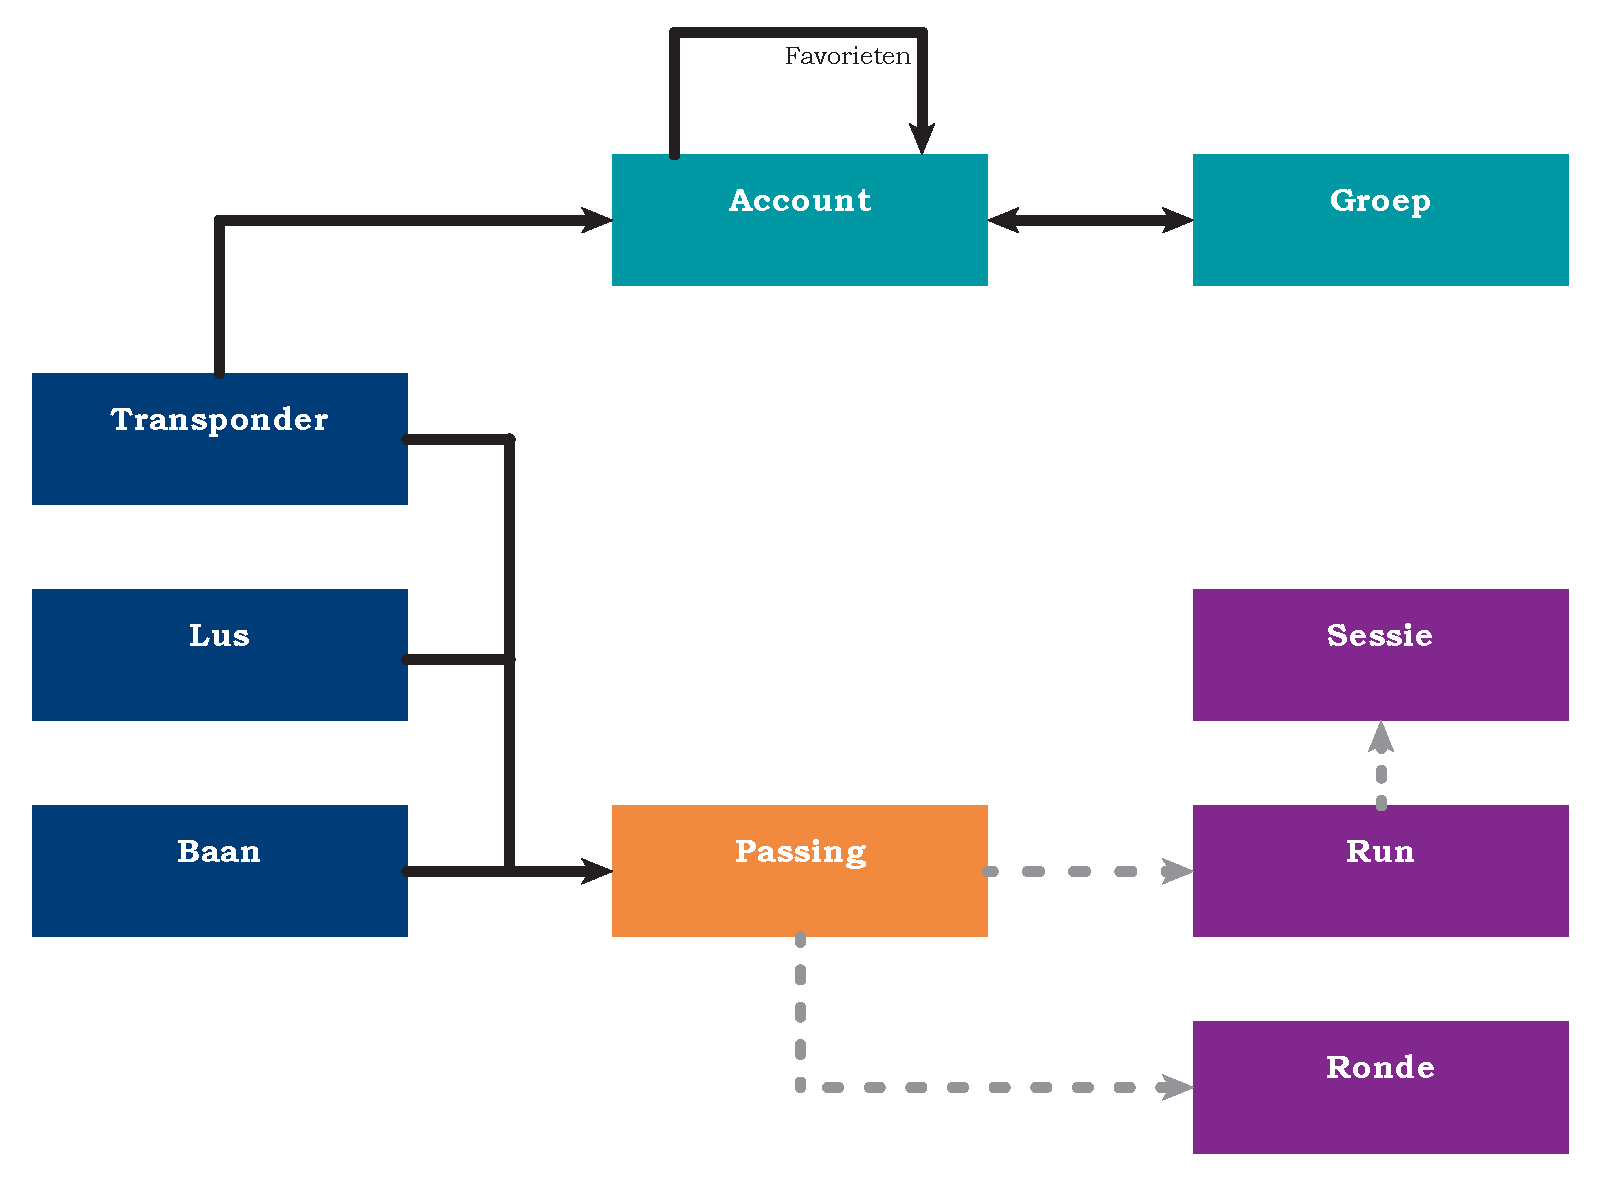
\includegraphics[width=.6\textwidth]{style/images/Entiteiten}    
  \end{center}
  \caption{De entiteiten en hun relaties.}
  \label{fig:entiteiten}
\end{figure}

Hoewel de daadwerkelijke structuur van de data in Azure Table Storage anders is dan in de figuur, geeft de figuur toch een goed beeld van deze entiteiten en hun relaties. 

\subsection{Azure SQL \& Entity Framework}
Azure SQL is de relationele SQL database van Azure en omdat de relaties in onze entiteiten worden beschreven door het Entity Framework~\cite{entityframework-msdn, entityframework-facto}, gebruikt onze applicatie de Entity Framework driver voor Azure SQL. Entity Framework is de defacto standaard voor relationele datalagen in ASP.NET. Het kan bijvoorbeeld relaties tussen entiteiten automatisch opzoeken. Ook hoeft er geen SQL code geschreven te worden, maar kan platformonafhankelijke LINQ code geschreven worden om entiteiten op te halen.

\subsection{Azure Table Storage}
De geaggregeerde data kan plat worden opgeslagen met behulp van NoSQL. Dit komt doordat alleen passings (doorkomsten), rondes en leaderboard-waarden entiteiten zijn in de aggregatie database. Zowel de sessie als het zijn van run of dan wel rust zijn eigenschappen van een ronde. De snelheid en segmenten worden niet opgeslagen.

Vanuit Emando ging de voorkeur voor het opslaan van de geaggregeerde data  uit naar de NoSQL Azure Table Storage. De Table Storage integreert eenvoudig met de reeds bestaande infrastructuur van het bedrijf. Bovendien biedt een gepartitioneerde en gesorteerde Table Storage tabel een groot performance voordeel: het goedkoop en snel kunnen selecteren van de laatste entiteiten per context.

Vanuit de Data Collector worden de doorkomsten die realtime binnen komen opgeslagen in Table Storage als backup. De structuur van deze tabel is terug te vinden in {\color{red} ref en tabel toevoegen }. Verderop in het aggregatieproces worden deze doorkomsten gekoppeld aan gebruikers. Deze aggregaties worden vervolgens opgeslagen in een aparte tabel binnen Azure Table Storage. De structuur van deze tabel is terug te vinden in {\color{red} ref en tabel toevoegen }.

Van snelheden, rondes, run/rust periodes en sessies worden leaderboards bijgehouden in Azure Table Storage. Deze hebben allen een eigen corresponderende tabel, zodat aggregaties parallel aan elkaar leaderboards kunnen updaten {\color{red} ref aggregatielaag }.
Alle leaderboards zijn voorzien van een leaderboard Id en een user Id. Het leaderboard Id houdt bij voor welke context het leaderboard geldig is. Dit kunnen banen, groepen, maar ook gebruikers zijn. Wanneer een gebruiker een ronde rijdt op een baan X, moeten zijn records voor de baan, zijn groepen en zijn eigen totalen geüpdatet worden. 

\begin{figure}[ht]
  \begin{center}
  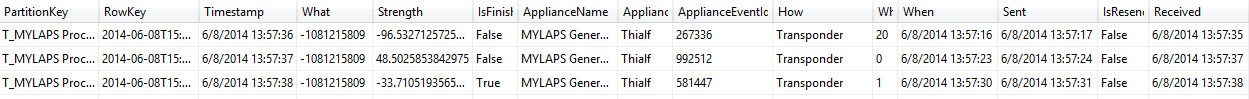
\includegraphics[width=.6\textwidth]{style/images/passingsStructure}    
  \end{center}
  \caption{De doorkomsten tabel met voorbeeld records. Hierbij is de Partition Key het type trasponder + transponder nummer en de Row Key het tijdstip waarop de doorkomst binnen kwam.}
  \label{fig:passingTableStructure}
\end{figure}

\begin{figure}[ht]
  \begin{center}
  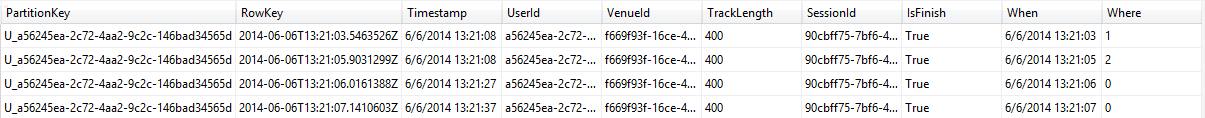
\includegraphics[width=.6\textwidth]{style/images/userPassingsStructure}    
  \end{center}
  \caption{De doorkomsten tabel met voorbeeld records. Hierbij is de Partition Key het account Id met een prefix voor gebruikers en de Row Key het tijdstip waarop de doorkomst binnen kwam.}
  \label{fig:userPassingTableStructure}
\end{figure}

\begin{figure}[ht]
  \begin{center}
  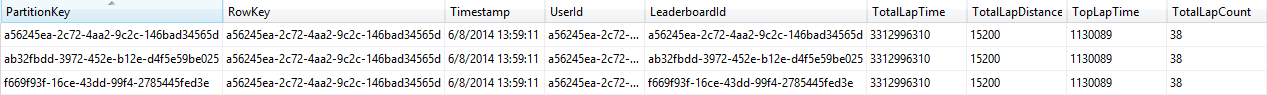
\includegraphics[width=.6\textwidth]{style/images/lapLeaderboardStructure}    
  \end{center}
  \caption{De ronde tabel met voorbeeld records. Hierbij is de Partition Key het account Id en de Row Key het ronde Id.}
  \label{fig:lapTableStructure}
\end{figure}

\begin{figure}[ht]
  \begin{center}
  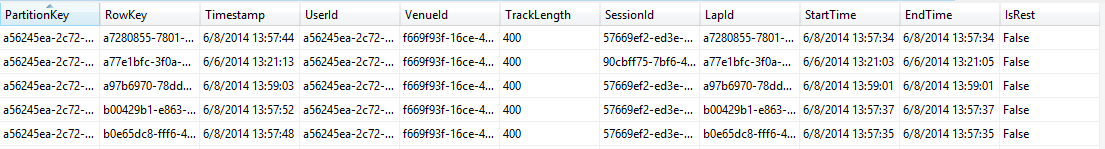
\includegraphics[width=.6\textwidth]{style/images/aggregationLapsStructure}    
  \end{center}
  \caption{De ronde leaderboard tabel, een voorbeeld van een leaderboard tabel. Hierbij is de Partition Key het account Id en de Row Key het context Id (groep, baan of account Id).}
  \label{fig:entiteiten}
\end{figure}

De structuur van de leaderboard tabellen ziet er als volgt uit.
{\color{red} tabel toevoegen}